%%%%%%%%%%%%%%%%%%%%%%%%%%%%%%%%%%%%%%%%%%%%%%%%%%%%%%%%%%%%%%%%%%%%%%%%%%%%%%%
%                       CARREGA DE LA CLASSE DE DOCUMENT                      %
%                                                                             %
% Les opcions admissibles son:                                                %
%      12pt / 11pt            (cos dels tipus de lletra; no feu servir 10pt)  %
%                                                                             %
% catalan/spanish/english     (llengua principal del treball)                 %
%                                                                             % 
% french/italian/german...    (si necessiteu fer servir alguna altra llengua) %
%                                                                             %
% listoffigures               (El document inclou un Index de figures)        %
% listoftables                (El document inclou un Index de taules)         %
% listofquadres               (El document inclou un Index de quadres)        %
% listofalgorithms            (El document inclou un Index d'algorismes)      %
%                                                                             %
%%%%%%%%%%%%%%%%%%%%%%%%%%%%%%%%%%%%%%%%%%%%%%%%%%%%%%%%%%%%%%%%%%%%%%%%%%%%%%%

\documentclass[11pt,english,listoffigures,listoftables]{tfgetsinf}

%%%%%%%%%%%%%%%%%%%%%%%%%%%%%%%%%%%%%%%%%%%%%%%%%%%%%%%%%%%%%%%%%%%%%%%%%%%%%%%
%                     CODIFICACIO DEL FITXER FONT                             %
%                                                                             %
%    windows fa servir normalment 'ansinew'                                   %
%    amb linux es possible que siga 'latin1' o 'latin9'                       %
%    Pero el mes recomanable es fer servir utf8 (unicode 8)                   %
%                                          (si el vostre editor ho permet)    % 
%%%%%%%%%%%%%%%%%%%%%%%%%%%%%%%%%%%%%%%%%%%%%%%%%%%%%%%%%%%%%%%%%%%%%%%%%%%%%%%

\usepackage[utf8]{inputenc} 

%%%%%%%%%%%%%%%%%%%%%%%%%%%%%%%%%%%%%%%%%%%%%%%%%%%%%%%%%%%%%%%%%%%%%%%%%%%%%%%
%                        ALTRES PAQUETS I DEFINICIONS                         %
%                                                                             %
% Carregueu aci els paquets que necessiteu i declareu les comandes i entorns  %
%                                          (aquesta seccio pot ser buida)     %
%%%%%%%%%%%%%%%%%%%%%%%%%%%%%%%%%%%%%%%%%%%%%%%%%%%%%%%%%%%%%%%%%%%%%%%%%%%%%%%

\usepackage{amsmath}
\usepackage{dsfont}
\usepackage{bbm}
\usepackage{tikz}
\usepackage{booktabs}
\tikzset{basic/.style={draw,fill=none,
                       text badly centered,minimum width=3em}}
\tikzset{input/.style={basic,circle,minimum width=3.5em}}
\tikzset{weights/.style={basic,rectangle,minimum width=2em}}
\tikzset{functions/.style={basic,circle, minimum width=4em}}
\newcommand{\addaxes}{\draw (0em,1em) -- (0em,-1em)
                            (-1em,0em) -- (1em,0em);}
\newcommand{\relu}{\draw[line width=1.5pt] (-1em,0) -- (0,0)
                                (0,0) -- (0.75em,0.75em);}
\newcommand{\stepfunc}{\draw[line width=1.5pt] (0.65em,0.65em) -- (0,0.65em) 
                                    -- (0,-0.65em) -- (-0.65em,-0.65em);}


\usetikzlibrary{decorations.pathreplacing}
\usetikzlibrary{fadings, fit, arrows.meta, shapes}
\usetikzlibrary{positioning,chains}
\newcommand{\empt}[2]{$#1^{\langle #2 \rangle}$}
%\DeclareMathOperator*{\argmax}{argmax}
%\DeclareMathOperator*{\argmin}{argmin}

%%%%%%%%%%%%%%%%%%%%%%%%%%%%%%%%%%%%%%%%%%%%%%%%%%%%%%%%%%%%%%%%%%%%%%%%%%%%%%%
%                        DADES DEL TREBALL                                    %
%                                                                             %
% titol, alumne, tutor i curs academic                                        %
%%%%%%%%%%%%%%%%%%%%%%%%%%%%%%%%%%%%%%%%%%%%%%%%%%%%%%%%%%%%%%%%%%%%%%%%%%%%%%%

\title{Adaptation of Large Language Models for Machine Translation tasks}
\author{Sergio Madrid Pérez}
\tutor{Alfons Juan Císcar \\ Jorge Civera Saiz}
% Director experimental (TO DO)
\curs{2023-2024}

%%%%%%%%%%%%%%%%%%%%%%%%%%%%%%%%%%%%%%%%%%%%%%%%%%%%%%%%%%%%%%%%%%%%%%%%%%%%%%%
%                     PARAULES CLAU/PALABRAS CLAVE/KEY WORDS                  %
%                                                                             %
% Independentment de la llengua del treball, s'hi han d'incloure              %
% les paraules clau i el resum en els tres idiomes                            %
%%%%%%%%%%%%%%%%%%%%%%%%%%%%%%%%%%%%%%%%%%%%%%%%%%%%%%%%%%%%%%%%%%%%%%%%%%%%%%%

\keywords{????, ?????????, ????, ?????????????????} % Paraules clau 
         {Aprendizaje Automático, Traducción Automática, modelo de lenguaje grande}              % Palabras clave
         {Machine Learning, Machine Translation, Large Language Model}        % Key words

%%%%%%%%%%%%%%%%%%%%%%%%%%%%%%%%%%%%%%%%%%%%%%%%%%%%%%%%%%%%%%%%%%%%%%%%%%%%%%%
%                              INICI DEL DOCUMENT                             %
%%%%%%%%%%%%%%%%%%%%%%%%%%%%%%%%%%%%%%%%%%%%%%%%%%%%%%%%%%%%%%%%%%%%%%%%%%%%%%%

\begin{document}

%%%%%%%%%%%%%%%%%%%%%%%%%%%%%%%%%%%%%%%%%%%%%%%%%%%%%%%%%%%%%%%%%%%%%%%%%%%%%%%
%              RESUMS DEL TFG EN VALENCIA, CASTELLA I ANGLES                  %
%%%%%%%%%%%%%%%%%%%%%%%%%%%%%%%%%%%%%%%%%%%%%%%%%%%%%%%%%%%%%%%%%%%%%%%%%%%%%%%

%\begin{abstract}
%????
%\end{abstract}
\begin{abstract}[spanish]
La traducción automática (MT, del inglés Machine Translation) es un campo importante dentro del aprendizaje automático, en el que el desarrollo de los modelos de lenguaje grandes ha demostrado tener un gran potencial para mejorar los sistemas actuales de traducción. Gracias a los modelos preentrenados que han aportado grandes empresas tecnológicas como Meta, Mistral AI o Google, la traducción automática multilingüe ha experimentado una notable mejora en los últimos años. En este contexto, este trabajo evaluará el rendimiento de los principales modelos de lenguaje grandes adaptados a tareas específicas de traducción en distintos pares de lenguas. Para ello, se hará uso de la infraestructura, datos y experiencia aportados por el grupo MLLP del VRAIN, adquiridos en el marco de proyectos de investigación y transferencia tecnológica desarrollados en los últimos años. 
\end{abstract}
\begin{abstract}[english]
Machine Translation (MT) is an important field within machine learning, where the development of large language models has shown great potential to improve current translation systems. Thanks to the pre-trained models provided by large technology companies such as Meta, Mistral AI or Google, multilingual machine translation has experienced a remarkable improvement in recent years. In this context, this work will evaluate the performance of the main large language models adapted to specific translation tasks in different language pairs. To this end, we will make use of data, technology, and expertise from the MLLP group of VRAIN, acquired within the framework of research and technology transfer projects developed in recent years.
\end{abstract}

%%%%%%%%%%%%%%%%%%%%%%%%%%%%%%%%%%%%%%%%%%%%%%%%%%%%%%%%%%%%%%%%%%%%%%%%%%%%%%%
%                              CONTINGUT DEL TREBALL                          %
%%%%%%%%%%%%%%%%%%%%%%%%%%%%%%%%%%%%%%%%%%%%%%%%%%%%%%%%%%%%%%%%%%%%%%%%%%%%%%%

\mainmatter

%%%%%%%%%%%%%%%%%%%%%%%%%%%%%%%%%%%%%%%%%%%%%%%%%%%%%%%%%%%%%%%%%%%%%%%%%%%%%%%
%                                  INTRODUCCIO                                %
%%%%%%%%%%%%%%%%%%%%%%%%%%%%%%%%%%%%%%%%%%%%%%%%%%%%%%%%%%%%%%%%%%%%%%%%%%%%%%%

\chapter{Introduction}

This work explores how the state-of-the-art Large Language Models (LLMs) perform in Machine Translation (MT) tasks. For this purpose, we will adapt some of the most popular LLMs and evaluate them using the standard metrics used in the field of MT. 

In this chapter, we describe the motivation and the main objectives of the work, as well as the key concepts that will be necessary for the reader to understand the rest of the work.

\section{Motivation}

In today's interconnected world, translation tools play an indispensable role in facilitating communication across linguistic barriers. Translation tools not only bridge language gaps but also democratize access to information, empowering individuals worldwide to have access to content in any language.

The exploration of machine translation through the adaptation of Large Language Models arises from a keen interest in leveraging cutting-edge technologies to enhance translations' quality. The decision of using LLMs for this work is based on their proven performance in numerous tasks, as well as on their accessibility through pre-trained models from leading technology companies.

\section{Objectives}

The main objectives of this work are the following:

\begin{enumerate}
    \item To adapt state-of-the-art LLMs and evaluate them on MT.
    \item To explore other methods for improving translations' quality.
    \item 
\end{enumerate}

\section{Document structure}

????? ????????????? ????????????? ????????????? ????????????? ????????????? 

\chapter{Background}

\section{Machine Learning}

The expansive field of Artificial Intelligence (AI) is in charge of building systems that enables computers and machines to simulate human intelligence and problem-solving capabilities. Whereas Machine Learning (ML) is a subset of AI that learns to make decisions by fitting mathematical models to observed data.

A popular definition of ML given by Tom Mitchell[] says the following:\\
%\indent
"A computer program is said to learn from experience E with respect to some class of tasks T and performance measure P, if its performance at tasks in T, as measured by P, improves with experience E."

Thus there are many different kinds of machine learning, depending on the nature of the tasks T we wish the system to learn, the nature of the performance measure P we use to evaluate the system, and the nature of the training signal or experience E we give it.

At its core, ML operates through statistical models, wherein the system's learning process entails the exploration of models that can generalize from a given dataset. This generalization enables the system to predict and produce desired outputs when presented with new input data, thus illustrating the essence of learning in ML.

Machine Learning tasks are typically classified based on the nature of the output they generate. In classification tasks, the objective is to predict the output \( y \) from a predefined set of \( C \) categories such that $y \in \{1, \ldots, \mathcal{C}\}$. Conversely, regression tasks aim to forecast outputs \( y \) that belong to a continuous range, such as $\mathbb{R}$.

Moreover, the training techniques used in ML can be classified into two main methods, depending on what data is available during training. Supervised learning uses a full set of labeled data during training, while in unsupervised learning the model is given unlabeled data, being able to discover patterns and insights without any explicit guidance or instruction.

In the context of this work, we will focus on adjusting pre-trained LLMs through supervised learning, which is the most popular training method in Natural Language Processing (NLP) tasks.
%Moreover, ML algorithms are delineated by the availability of output labels during training, giving rise to %various learning paradigms.
%Machine Learning (ML) stands at the forefront of %Artificial Intelligence (AI) and refers to the automated detection of meaningful patterns in data

\subsection{Supervised Learning}

The most common form of ML is supervised learning. In this problem, the task \( T \) is to learn a mapping \( f \) from inputs $x \in \mathcal{X}$ to outputs $y \in \mathcal{Y}$. The inputs \( x \) are also called features and normally consist of a fixed-dimensional vector of numbers. The output \( y \) is also known as label or target. The experience \( E \) is presented in the form of a set of \( N \) input-output tuples $\mathcal{D}=\{( x_{n},y_{n} )\}_{n=1}^N$, known as the training set.

Thus, the model is just a mathematical function $f(x,\theta)$ whose parameters \( \theta \) are often adjusted during the learning process, which usually consists in minimizing a loss function  \( L \) over the training set. 

\begin{equation}
\hat\theta=\underset{x}{\arg\max}
\end{equation}

In classification problems, the goal of supervised learning is to automatically come up with a model so as to reliably predict the labels for any given input. In these problems, the performance can be measured in terms of the misclassification rate on the training set:

\begin{equation}
\mathcal{L}(\theta)\overset{\Delta}{=}\frac{1}{N}\sum_{n=1}^{N}\mathbbm{I}(y_n\neq f(x_n,\theta))
\end{equation}

where \( \mathbbm{I} \) is the indicator function:

\begin{equation}
\mathbb{I}(e) = 
\begin{cases} 
1 & \text{if } e \text{ is true} \\ 
0 & \text{if } e \text{ is false} 
\end{cases}
\end{equation}

TO-DO: Regression problems, Gradiend descent

\subsection{Neural Networks}

Neural networks are a cornerstone of modern machine learning, inspired by the biological neural networks present in animal brains. These computational models consist of layers of interconnected nodes, or neurons, which process and transmit information. The architecture of neural networks allows them to learn complex patterns in data, making them suitable for a wide range of tasks like image recognition or natural language processing.

A neural network (NN) is composed of an input layer, one or more hidden layers and an output layer. Each layer consists of nodes and each node is connected to every node in the subsequent layer. The connections between nodes have associated weights, which are adjusted during training to optimize the network's performance.

The Perceptron is one of the simplest and most fundamental types of neural networks, introduced by Franck Rosenblatt in 1958. It serves as the building block for more complex neural network architectures. The Perceptron is a linear classifier for binary classification tasks.

\begin{figure}
    \centering
%    \caption{Caption}
%    \label{fig:perceptron}
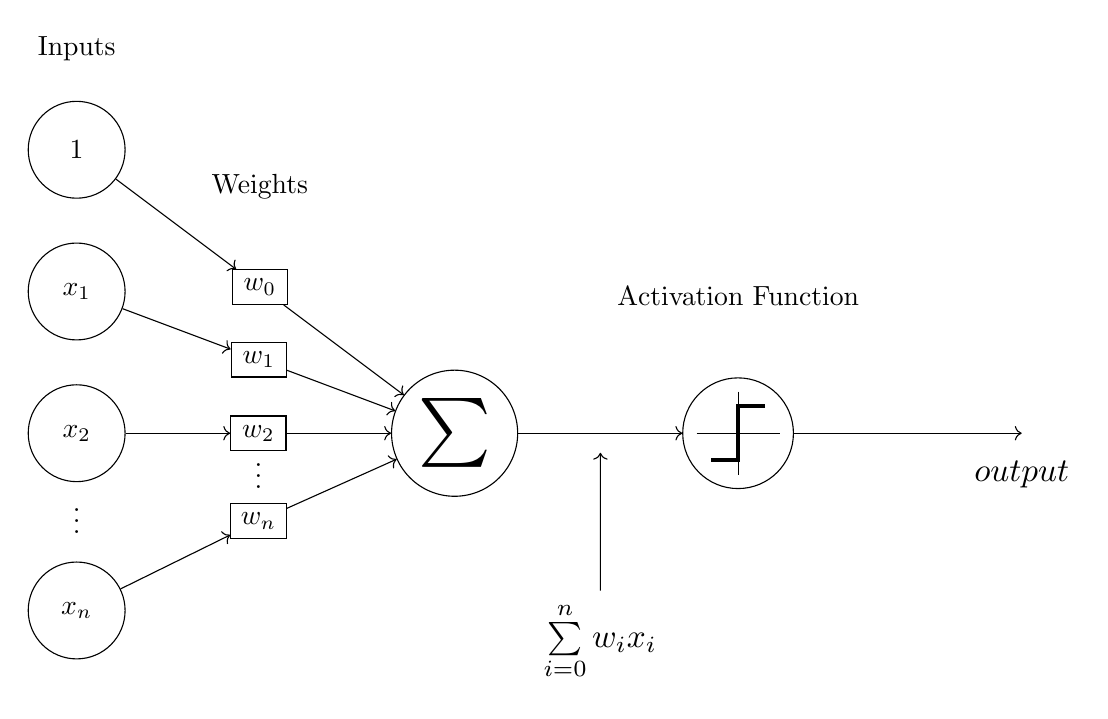
\begin{tikzpicture}[scale=1.2]
    % Draw input nodes
    \foreach \h [count=\hi ] in {$x_2$,$x_1$,$1$}{%
        \node[input] (f\hi) at (0,\hi*1.5cm-1.5 cm) {\h};
      }
    % Dot dot dot ... x_n
    \node[below=0.62cm] (idots) at (f1) {\vdots};
    \node[input, below=0.62cm] (last_input) at (idots) {$x_n$};
    % Draw summation node
    \node[functions] (sum) at (4,0) {\Huge$\sum$};
    % Draw edges from input nodes to summation node
    \foreach \h [count=\hi ] in {$w_2$,$w_1$,$w_0$}{%
          \path (f\hi) -- node[weights] (w\hi) {\h} (sum);
          \draw[->] (f\hi) -- (w\hi);
          \draw[->] (w\hi) -- (sum);
        }
    % Dot dot dot ... w_n
    \node[below=0.05cm] (wdots) at (w1) {\vdots};
    \node[weights, below=0.45cm] (last_weight) at (wdots) {$w_n$};
    % Add edges for last node and last weight etc
    \path[draw,->] (last_input) -- (last_weight);
    \path[draw,->] (last_weight) -- (sum);
    % Draw node for activation function
    \node[functions] (activation) at (7,0) {};
    % Place activation function in its node
    \begin{scope}[xshift=7cm,scale=1.25]
        \addaxes
        % flexible selection of activation function
        % \relu
        \stepfunc
    \end{scope}
    % Connect sum to activation function
    \draw[->] (sum) -- (activation) node (sum_eq) [midway, below=2cm, scale=1.2] {$\sum\limits_{i=0}^n w_ix_i$} node (sum_activation_midway) [midway, below] {};
    \path[draw,->] (sum_eq) -- (sum_activation_midway);
    \draw[->] (activation) -- ++(3,0) node (perceptron_output) [below=0.2cm, scale=1.2] {$output$};
    % Labels
    \node[above=1cm]  at (f3) {Inputs};
    \node[above=1cm] at (w3) {Weights};
    \node[above=1.5cm] at (activation) {Activation Function};
\end{tikzpicture}
\caption{Single-Layer Perceptron}
\label{fig:perceptron}
\end{figure}
%From: https://tex.stackexchange.com/questions/104334/tikz-diagram-of-a-perceptron

As show in Figure , the original Perceptron consists of a single neuron that takes as input a vector of features \( x \) and outputs a single value \( y \). The output is computed by the following equation:

\begin{equation}
    y = g(z) = 
    \begin{cases}
        1 & \text{ if } z \ge 0 \\
        0 & \text{otherwise}
    \end{cases}
\end{equation}

\begin{equation}
    z = \sum_{i=0}^n\theta_ix_i = \theta^{t}x
\end{equation}


where:
\begin{itemize}
    \item x is an n-dimensional input vector of features, whose component \( x_0 \) is usually fixed to one.
    \item \( \theta \) is the vector containing the weights of the neuron. The weight \( \theta_0 \) is also know as bias.
    \item $g(\cdot)$ is an activation function used for selecting the class of the target.
\end{itemize}

Thus, the Perceptron is a binary classifier, in other words, it is an algorithm that classifies input by separating two classes with a straight line. The learning algorithm used for adjusting the weights of the Perceptron can be summarized in the following steps:

\begin{enumerate}
    \item Start by initializing the vector of weights to random values.
    \item For each training sample \( x_i \), compute output \( \hat{y}_i \) with the current vector of weights.
    \item If the Perceptron makes an incorrect prediction, update the weights according to the following formula:
    \begin{equation}
        \theta_{i} = \theta_i - \lambda(\hat{y}_t-y_t)x_t
    \end{equation}
    where \( \lambda \) is the learning rate, \( \hat{y} \) is the predicted output and \( y \) is the actual output.
    \item Repeat steps 2 and 4 for a fixed number of epochs or until the model converges. An epoch is one complete pass through the entire dataset.

\end{enumerate}

The convergence of the Perceptron is only guaranteed if the two classes are linearly separable. If the data is not linearly separable, the algorithm will not converge and the weights will oscilate indefinitely.

The XOR Problem, introduced in the book Perceptrons[], is a classic example of a non-linearly separable problem, which consists in predicting the output of XOR logic gates. This problem illustrates the limitations of the Perceptron.



\begin{figure}
\centering
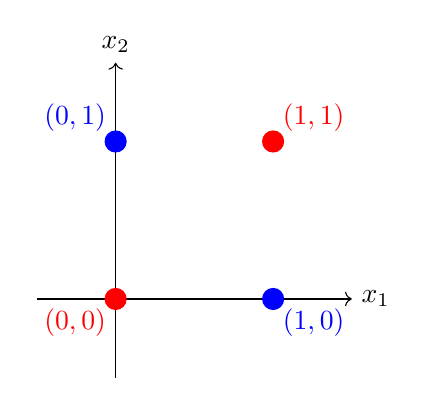
\begin{tikzpicture}[scale=2]
    % Axes
    \draw[->] (-0.5,0) -- (1.5,0) node[right] {$x_1$};
    \draw[->] (0,-0.5) -- (0,1.5) node[above] {$x_2$};
    
    % Points for Class 1 (0,1) and (1,0)
    \fill[blue] (0,1) circle (2pt) node[above left] {$(0,1)$};
    \fill[blue] (1,0) circle (2pt) node[below right] {$(1,0)$};
    
    % Points for Class 2 (0,0) and (1,1)
    \fill[red] (0,0) circle (2pt) node[below left] {$(0,0)$};
    \fill[red] (1,1) circle (2pt) node[above right] {$(1,1)$};

    % Labels for classes
    \node[blue] at (-0.5, 1.2){};
    \node[red] at (1.5, 1.2) {};

    % Grid lines for reference
    %\draw[dashed, gray] (0,0) grid (1,1);
    
    % Optional: Lines connecting points to form a square
    %\draw[gray] (0,0) -- (0,1) -- (1,1) -- (1,0) -- cycle;

\end{tikzpicture}
\caption{Graph representing the XOR problem with two classes.}
\label{fig:xor}
\end{figure}

\begin{figure}
    \centering
    \begin{tabular}{|c|c|c|}
        \hline
        $x_1$ & $x_2$ & $y = x_1 \oplus x_2$ \\
        \hline
        0 & 0 & 0 \\
        0 & 1 & 1 \\
        1 & 0 & 1 \\
        1 & 1 & 0 \\
        \hline
    \end{tabular}
    \caption{Truth table for the XOR gate.}
    \label{fig:xor_table}
\end{figure}

To address the limitations of the basic Perceptron, more advanced models have been developed. The most popular one is the Multi-Layer Perceptron (MLP), which consists of an input layer, one or more hidden layers and an output layer (see Figure ). The hidden layers enable the network to learn complex, non-linear relationships between inputs and outputs.

\begin{figure}[h]
	\centering
	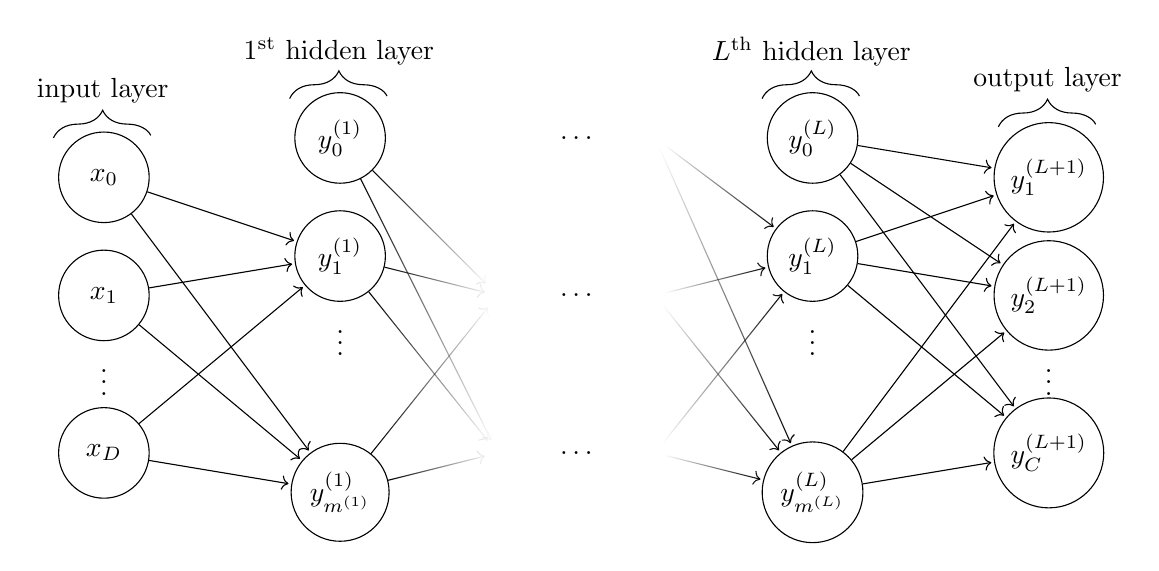
\begin{tikzpicture}[shorten >=1pt]
		\tikzstyle{unit}=[draw,shape=circle,minimum size=1.15cm]
		%\tikzstyle{hidden}=[draw,shape=circle,fill=black!25,minimum size=1.15cm]
		\tikzstyle{hidden}=[draw,shape=circle,minimum size=1.15cm]

		\node[unit](x0) at (0,3.5){$x_0$};
		\node[unit](x1) at (0,2){$x_1$};
		\node at (0,1){\vdots};
		\node[unit](xd) at (0,0){$x_D$};

		\node[hidden](h10) at (3,4){$y_0^{(1)}$};
		\node[hidden](h11) at (3,2.5){$y_1^{(1)}$};
		\node at (3,1.5){\vdots};
		\node[hidden](h1m) at (3,-0.5){$y_{m^{(1)}}^{(1)}$};

		\node(h22) at (5,0){};
		\node(h21) at (5,2){};
		\node(h20) at (5,4){};
		
		\node(d3) at (6,0){$\ldots$};
		\node(d2) at (6,2){$\ldots$};
		\node(d1) at (6,4){$\ldots$};

		\node(hL12) at (7,0){};
		\node(hL11) at (7,2){};
		\node(hL10) at (7,4){};
		
		\node[hidden](hL0) at (9,4){$y_0^{(L)}$};
		\node[hidden](hL1) at (9,2.5){$y_1^{(L)}$};
		\node at (9,1.5){\vdots};
		\node[hidden](hLm) at (9,-0.5){$y_{m^{(L)}}^{(L)}$};

		\node[unit](y1) at (12,3.5){$y_1^{(L+1)}$};
		\node[unit](y2) at (12,2){$y_2^{(L+1)}$};
		\node at (12,1){\vdots};	
		\node[unit](yc) at (12,0){$y_C^{(L+1)}$};

		\draw[->] (x0) -- (h11);
		\draw[->] (x0) -- (h1m);

		\draw[->] (x1) -- (h11);
		\draw[->] (x1) -- (h1m);

		\draw[->] (xd) -- (h11);
		\draw[->] (xd) -- (h1m);

		\draw[->] (hL0) -- (y1);
		\draw[->] (hL0) -- (yc);
		\draw[->] (hL0) -- (y2);

		\draw[->] (hL1) -- (y1);
		\draw[->] (hL1) -- (yc);
		\draw[->] (hL1) -- (y2);

		\draw[->] (hLm) -- (y1);
		\draw[->] (hLm) -- (y2);
		\draw[->] (hLm) -- (yc);

		\draw[->,path fading=east] (h10) -- (h21);
		\draw[->,path fading=east] (h10) -- (h22);
		
		\draw[->,path fading=east] (h11) -- (h21);
		\draw[->,path fading=east] (h11) -- (h22);
		
		\draw[->,path fading=east] (h1m) -- (h21);
		\draw[->,path fading=east] (h1m) -- (h22);
		
		\draw[->,path fading=west] (hL10) -- (hL1);
		\draw[->,path fading=west] (hL11) -- (hL1);
		\draw[->,path fading=west] (hL12) -- (hL1);
		
		\draw[->,path fading=west] (hL10) -- (hLm);
		\draw[->,path fading=west] (hL11) -- (hLm);
		\draw[->,path fading=west] (hL12) -- (hLm);
		
		\draw [decorate,decoration={brace,amplitude=10pt},xshift=-4pt,yshift=0pt] (-0.5,4) -- (0.75,4) node [black,midway,yshift=+0.6cm]{input layer};
		\draw [decorate,decoration={brace,amplitude=10pt},xshift=-4pt,yshift=0pt] (2.5,4.5) -- (3.75,4.5) node [black,midway,yshift=+0.6cm]{$1^{\text{st}}$ hidden layer};
		\draw [decorate,decoration={brace,amplitude=10pt},xshift=-4pt,yshift=0pt] (8.5,4.5) -- (9.75,4.5) node [black,midway,yshift=+0.6cm]{$L^{\text{th}}$ hidden layer};
		\draw [decorate,decoration={brace,amplitude=10pt},xshift=-4pt,yshift=4pt] (11.5,4) -- (12.75,4) node [black,midway,yshift=+0.6cm]{output layer};
	\end{tikzpicture}
	\caption[Network graph for a $(L+1)$-layer perceptron.]{Network graph of a $(L+1)$-layer perceptron with $D$ input units and $C$ output units. The $l^{\text{th}}$ hidden layer contains $m^{(l)}$ hidden units.}
	\label{fig:multilayer-perceptron}
\end{figure}
%From https://github.com/davidstutz/latex-resources/blob/master/tikz-multilayer-perceptron/multilayer-perceptron.tex


In a MLP, each neuron in a given layer is fully connected to the neurons in the previous and subsequent layers, meaning that every neuron in one layer receives inputs from all the neurons in the previous layer and sends its output to all neurons in the next layer. The equation defined by the MLP can be expressed as:

\begin{equation}
    s_j^l = g(\sum_{i=0}^{M_{l-1}}\theta_{ji}^l \cdot s_i^{l-1}), 1 \leq j \leq M_l, 1 \leq l \leq L
\end{equation}

Activation functions \( g(\cdot)\) introduce non-linearity into the MLP and allow it to deal with non-linear decision boundaries. Some examples of activation functions are the ReLU[], the Sigmoid or the hyperbolic tangent.

The learning process of an MLP is typically carried out using the backpropagation algorithm combined with an optimization technique such as gradient descent. The formula for updating the weights of the network can be expressed as:

\begin{equation}
    \Delta \theta_{ij}^l=-\lambda \frac{\partial L(\theta)}{\partial \theta_{ij}^l}
\end{equation}

where \( L(\theta) \) is the loss function we want to optimize. The choice of this loss function depends on the nature of the task.

In classification problems with C classes, the most common is the Cross-Entropy Loss. This function measures the difference between two probability distributions.

\begin{equation}
    L(\theta) = - \sum_{c=1}^Cy_clog(\hat{y}_k)
\end{equation}

On the other hand, in regression problems the most common loss functions are the Mean Squared Error (MSE) and the Mean Absolute Error (MAE).

\begin{equation}
    MSE = \frac{1}{N} \sum_{i=1}^{N} (y_i - \hat{y}_i)^2
\end{equation}

\begin{equation}
    MAE = \frac{1}{N} \sum_{i=1}^{N} |y_i - \hat{y}_i|
\end{equation}

A neural network without loops, where the information can only flow in one direction forming a directed acyclic graph (DAG), is known as Feedforward Neural Network (FNN). The main limitation of this kind of networks is their inability to maintain context or memory of past inputs, as each input is processed independently. To overcome this problem, Recurrent Neural Networks (RNNs) were introduced[]. This kind of neural network maps from an input space of sequences to an output space of sequences in a stateful way. That is, the prediction \( y_t \) at instant \( t \) depends not only on the input \( x_t \), but also on the current hidden state of the system \( h_t \), which is updated over time, as the sequence is processed. 

\begin{figure}[h]
    \centering
    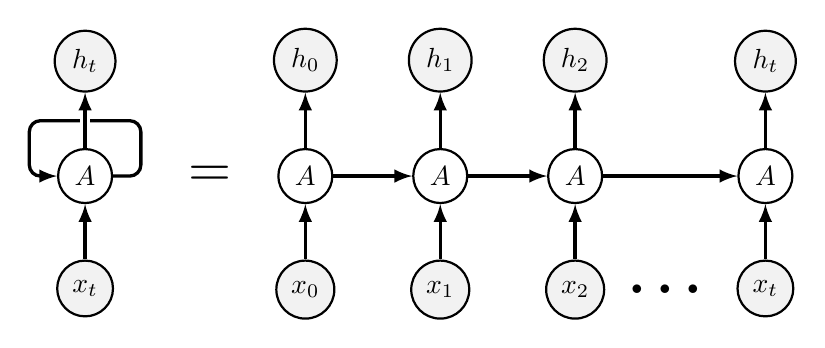
\begin{tikzpicture}[item/.style={circle,draw,thick,align=center},
    itemc/.style={item,on chain,join}]
        \begin{scope}[start chain=going right,nodes=itemc,every join/.style={-latex,very thick},local bounding box=chain]
            \path node (A0) {$A$} 
                  node (A1) {$A$} 
                  node (A2) {$A$} 
                  node[xshift=2em] (At) {$A$};
        \end{scope}
        \node[left=1em of chain,scale=2] (eq) {$=$};
        \node[left=2em of eq,item] (AL) {$A$};
        \path (AL.west) ++ (-1em,2em) coordinate (aux);
        \draw[very thick,-latex,rounded corners] (AL.east) -| ++ (1em,2em) -- (aux) |- (AL.west);
        \foreach \X in {0,1,2,t} {
            \draw[very thick,-latex] (A\X.north) -- ++ (0,2em) node[above,item,fill=gray!10] (h\X) {$h_\X$};
            \draw[very thick,latex-] (A\X.south) -- ++ (0,-2em) node[below,item,fill=gray!10] (x\X) {$x_\X$};
        }
        \draw[white,line width=0.8ex] (AL.north) -- ++ (0,1.9em);
        \draw[very thick,-latex] (AL.north) -- ++ (0,2em) node[above,item,fill=gray!10] {$h_t$};
        \draw[very thick,latex-] (AL.south) -- ++ (0,-2em) node[below,item,fill=gray!10] {$x_t$};
        \path (x2) -- (xt) node[midway,scale=2,font=\bfseries] {\dots};
    \end{tikzpicture}
    \caption{Illustration of a recurrent neural network structure with hidden states and inputs.}
    \label{fig:rnn_structure}
\end{figure}
%https://tex.stackexchange.com/questions/494139/how-do-i-draw-a-simple-recurrent-neural-network-with-goodfellows-style

The main drawback of RNNs is that they struggle to capture long-term dependencies in input sequences. During backpropagation, gradients are propagated from the last neuron all the way to the first one. The repeated multiplication of gradients through the hidden states can result in gradient vanishing or exploding, that is, gradients can become extremely small or large.

In order to tackle these limitations, the Long-Short Term Memory (LSTM) networks were introduced. They are a type of RNN that introduce a more sophisticated architecture enabling them to maintain information over longer periods, making them particularly effective for tasks involving sequential data, such as NLP.

LSTMs units are commonly composed of a memory cell, an input gate, an output gate and a forget gate. The cells remembers values over time and the three gates regulate the flow of information into and out of the cell. The input gate determines what new information is stored in the cell current state. In contrast, the forget gate decides what information is discarded from the cell state. Finally, the output gate controls what information from the cell state is used as the output.

\begin{figure}[ht]
    \centering
    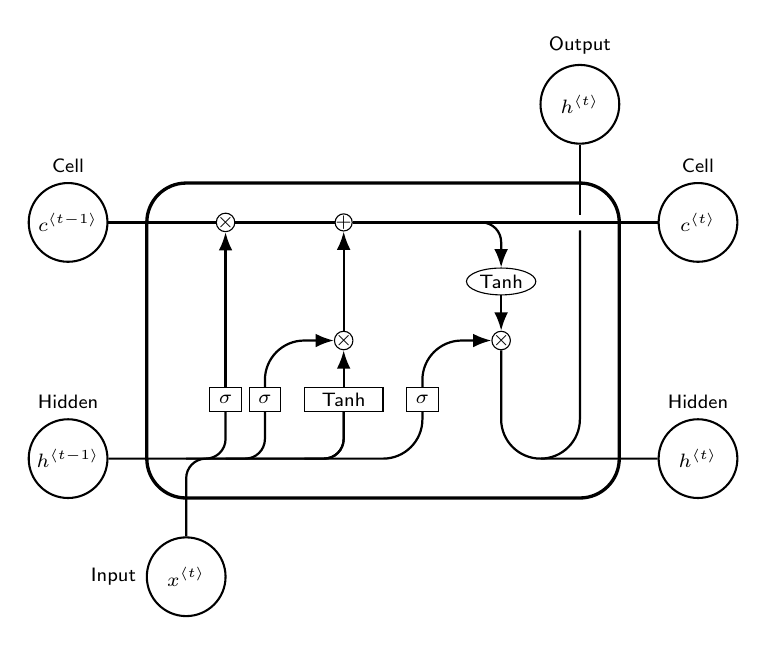
\begin{tikzpicture}[
        font=\sf \scriptsize,
        >=LaTeX,
        cell/.style={
            rectangle, 
            rounded corners=5mm, 
            draw,
            very thick,
        },
        operator/.style={
            circle,
            draw,
            inner sep=-0.5pt,
            minimum height =.2cm,
        },
        function/.style={
            ellipse,
            draw,
            inner sep=1pt
        },
        ct/.style={
            circle,
            draw,
            line width = .75pt,
            minimum width=1cm,
            inner sep=1pt,
        },
        gt/.style={
            rectangle,
            draw,
            minimum width=4mm,
            minimum height=3mm,
            inner sep=1pt
        },
        mylabel/.style={
            font=\scriptsize\sffamily
        },
        ArrowC1/.style={
            rounded corners=.25cm,
            thick,
        },
        ArrowC2/.style={
            rounded corners=.5cm,
            thick,
        },
    ]

    % Drawing starts here
    \node [cell, minimum height =4cm, minimum width=6cm] {}; 

    % Draw inputs named ibox#
    \node [gt] (ibox1) at (-2,-0.75) {$\sigma$};
    \node [gt] (ibox2) at (-1.5,-0.75) {$\sigma$};
    \node [gt, minimum width=1cm] (ibox3) at (-0.5,-0.75) {Tanh};
    \node [gt] (ibox4) at (0.5,-0.75) {$\sigma$};

   % Draw operators   named mux# , add# and func#
    \node [operator] (mux1) at (-2,1.5) {$\times$};
    \node [operator] (add1) at (-0.5,1.5) {+};
    \node [operator] (mux2) at (-0.5,0) {$\times$};
    \node [operator] (mux3) at (1.5,0) {$\times$};
    \node [function] (func1) at (1.5,0.75) {Tanh};

    % Draw External inputs, named as basis c,h,x
    \node[ct, label={[mylabel]Cell}] (c) at (-4,1.5) {\empt{c}{t-1}};
    \node[ct, label={[mylabel]Hidden}] (h) at (-4,-1.5) {\empt{h}{t-1}};
    \node[ct, label={[mylabel]left:Input}] (x) at (-2.5,-3) {\empt{x}{t}};

    % Draw External outputs, named as basis c2,h2,x2
    \node[ct, label={[mylabel]Cell}] (c2) at (4,1.5) {\empt{c}{t}};
    \node[ct, label={[mylabel]Hidden}] (h2) at (4,-1.5) {\empt{h}{t}};
    \node[ct, label={[mylabel]Output}] (x2) at (2.5,3) {\empt{h}{t}};
    
% Start connecting all.
    %Intersections and displacements are used. 
    % Drawing arrows    
    \draw [ArrowC1] (c) -- (mux1) -- (add1) -- (c2);

    % Inputs
    \draw [ArrowC2] (h) -| (ibox4);
    \draw [ArrowC1] (h -| ibox1)++(-0.5,0) -| (ibox1); 
    \draw [ArrowC1] (h -| ibox2)++(-0.5,0) -| (ibox2);
    \draw [ArrowC1] (h -| ibox3)++(-0.5,0) -| (ibox3);
    \draw [ArrowC1] (x) -- (x |- h)-| (ibox3);

    % Internal
    \draw [->, ArrowC2] (ibox1) -- (mux1);
    \draw [->, ArrowC2] (ibox2) |- (mux2);
    \draw [->, ArrowC2] (ibox3) -- (mux2);
    \draw [->, ArrowC2] (ibox4) |- (mux3);
    \draw [->, ArrowC2] (mux2) -- (add1);
    \draw [->, ArrowC1] (add1 -| func1)++(-0.5,0) -| (func1);
    \draw [->, ArrowC2] (func1) -- (mux3);

    %Outputs
    \draw [-, ArrowC2] (mux3) |- (h2);
    \draw (c2 -| x2) ++(0,-0.1) coordinate (i1);
    \draw [-, ArrowC2] (h2 -| x2)++(-0.5,0) -| (i1);
    \draw [-, ArrowC2] (i1)++(0,0.2) -- (x2);

    \end{tikzpicture}
    \caption{Architecture of an LSTM unit.}
    \label{fig:lstm_architecture}
\end{figure}
\section{Transformers}

%The transformer architecture represent a revolutionary architecture in the field of deep learning, particularly in NLP. It has 

Transformers represent a revolution in the field of deep learning, particularly in NLP, by introducing a powerful architecture that excels in handling sequential data and capturing long-range dependencies. Unlike traditional recurrent neural networks (RNNs) and their variants, transformers rely on self-attention mechanisms that allow them to process all elements of a sequence simultaneously, rather than sequentially. This innovation enables transformers to model complex patterns and relationships within data.

\subsection{Self-attention}



\section{Machine Translation}

\section{Large Language Models}

%\section{Notes bibliografiques} %%%%% Opcional

%????? ????????????? ????????????? ????????????? ????????????? ?????????????

%%%%%%%%%%%%%%%%%%%%%%%%%%%%%%%%%%%%%%%%%%%%%%%%%%%%%%%%%%%%%%%%%%%%%%%%%%%%%%%
%                         CAPITOLS (tants com calga)                          %
%%%%%%%%%%%%%%%%%%%%%%%%%%%%%%%%%%%%%%%%%%%%%%%%%%%%%%%%%%%%%%%%%%%%%%%%%%%%%%%

\chapter{Adaptation of LLMs for MT}

This chapter delves into the comparative analysis of some of the most popular publicly available LLMs when adapted for MT tasks. For this study, we will train and evaluate all models for \( en \rightarrow es\) and \( en \rightarrow de\) language pairs. Thus, our main goal is to find out which LLMs performs best for each language pair and to determine whether LLMs are suitable for MT tasks.

\section{Datasets}

\section{Multilingual Encoder-Decoder Models}

\begin{table}
    \centering
    \textbf{Interact: en $\rightarrow$ es, de \\}
    \scalebox{1}{
    \begin{tabular}{l c c c c c c}
        \toprule
        {} & {} & \multicolumn{2}{c}{Spanish} & {} & \multicolumn{2}{c}{German} \\ \cmidrule{3-7} 
        Model & LORA & BLEU & COMET & {} & BLEU & COMET \\
        \midrule \midrule
        NLLB-600M & No & 55.3 & 86.05 & {} & 37.3 & 82.21 \\
        NLLB-1.3B & No & 55.9 & 86.22 & {} & 39.3 & 82.92 \\
        NLLB-3.3B & No & 56.3 & 86.34 & {} & 41.1 & 83.50 \\
        \midrule
        NLLB-600M & Yes & 55.4 & 86.44 & {} & 38.2 & 83.03 \\
        NLLB-1.3B & Yes & \textbf{57.3} & 87.09 & {} & 41.2 & 84.46 \\
        NLLB-3.3B & Yes & \textbf{57.3} & \textbf{87.23} & {} & \textbf{42.8} & \textbf{84.88} \\ 
        \bottomrule
    \end{tabular}
    }
    \caption{BLEU and COMET scores for encoder-decorder models on Interact test set}
    \label{tab:results_nllb_interact}
\end{table}

\begin{table}
    \centering
    \textbf{Europarl-ST : en $\rightarrow$ es, de \\}
    \scalebox{1}{
    \begin{tabular}{l c c c c c c}
        \toprule
        {} & {} & \multicolumn{2}{c}{Spanish} & {} & \multicolumn{2}{c}{German} \\ \cmidrule{3-7} 
        Model & LORA & BLEU & COMET & {} & BLEU & COMET \\
        \midrule \midrule
        NLLB-600M & No & 44.4 & 88.56 & {} & 31.4 & 86.84 \\ 
        NLLB-1.3B & No & 46.2 & 88.97 & {} & 33.4 & 87.35 \\
        NLLB-3.3B & No & 47.3 & 89.36 & {} & 35.1 & 88.10 \\
        \midrule
        NLLB-600M & Yes & 46.7 & 88.69 & {} & 35.3 & 87.63 \\
        NLLB-1.3B & Yes & 48.0 & 89.27 & {} & 37.2 & 88.33 \\
        NLLB-3.3B & Yes & \textbf{49.0} & \textbf{89.38} & {} & \textbf{38.5} & \textbf{88.83} \\ 
        \bottomrule
    \end{tabular}
    }
    \caption{BLEU and COMET scores for encoder-decorder models on Europarl-ST test set}
    \label{tab:results_nllb_europarl}
\end{table}

\section{Multilingual Decoder-Only Models}

\begin{table}
    \centering
    \textbf{Interact: en $\rightarrow$ es, de \\}
    \scalebox{1}{
    \begin{tabular}{l c c c c c}
        \toprule
        {} & \multicolumn{2}{c}{Spanish} & {} & \multicolumn{2}{c}{German} \\ \cmidrule{2-6} 
        Model & BLEU & COMET & {} & BLEU & COMET \\
        \midrule \midrule
        Llama2-7B & 51.0 & 86.18 & {} & 33.5 & 83.40 \\
        Gemma-7B & 50.8 & 85.77 & {} & 34.7 & 83.91 \\
        Falcon-7B & 49.5 & 85.99 & {} & 33.4 & 83.12 \\
        Mistral-7B & 50.6 & 86.21 & {} & 34.7 & 83.81 \\
        Llama3-8B & \textbf{52.1} & \textbf{86.37} & {} & \textbf{36.1} & \textbf{84.19} \\
        \bottomrule
    \end{tabular}
    }
    \caption{BLEU and COMET scores for decoder-only models on Interact test set.}
    \label{tab:results_decoder_only_interact}
\end{table}

\begin{table}
    \centering
    \textbf{Europarl-ST: en $\rightarrow$ es, de \\}
    \scalebox{1}{
    \begin{tabular}{l c c c c c}
        \toprule
        {} & \multicolumn{2}{c}{Spanish} & {} & \multicolumn{2}{c}{German} \\ \cmidrule{2-6} 
        Model & BLEU & COMET & {} & BLEU & COMET \\
        \midrule \midrule
        Llama2-7B & 46.7 & 89.33 & {} & 34.6 & 88.26 \\
        Gemma-7B & 46.6 & 89.15 & {} & 34.5 & 88.20 \\
        Falcon-7B & 46.0 & 89.06 & {} & 33.5 & 87.64 \\
        Mistral-7B & 46.8 & 89.46 & {} & 34.5 & 88.41 \\
        Llama3-8B & \textbf{47.5} & \textbf{89.50} & {} & \textbf{35.6} & \textbf{88.46} \\
        \bottomrule
    \end{tabular}
    }
    \caption{BLEU and COMET scores for decoder-only models on Europarl-ST test set.}
    \label{tab:results_decoder_only_europarl}
\end{table}

\chapter{}

????? ????????????? ????????????? ????????????? ????????????? ????????????? 

\section{?? ???? ???? ? ?? ??}

????? ????????????? ????????????? ????????????? ????????????? ?????????????

%%%%%%%%%%%%%%%%%%%%%%%%%%%%%%%%%%%%%%%%%%%%%%%%%%%%%%%%%%%%%%%%%%%%%%%%%%%%%%%
%                                 CONCLUSIONS                                 %
%%%%%%%%%%%%%%%%%%%%%%%%%%%%%%%%%%%%%%%%%%%%%%%%%%%%%%%%%%%%%%%%%%%%%%%%%%%%%%%

\chapter{Conclusions}

????? ????????????? ????????????? ????????????? ????????????? ????????????? 

%%%%%%%%%%%%%%%%%%%%%%%%%%%%%%%%%%%%%%%%%%%%%%%%%%%%%%%%%%%%%%%%%%%%%%%%%%%%%%%
%                                BIBLIOGRAFIA                                 %
%%%%%%%%%%%%%%%%%%%%%%%%%%%%%%%%%%%%%%%%%%%%%%%%%%%%%%%%%%%%%%%%%%%%%%%%%%%%%%%

\begin{thebibliography}{10}

%%%%%%%%%%%%%%%%%%%%%%%%%%%%%%%%%%%%%%%%%%%%%%%%%%%%%%%%%%%%%%%%%%%%%%%%%%%%%%%
% MODEL D'ARTICLE                                                             %
%%%%%%%%%%%%%%%%%%%%%%%%%%%%%%%%%%%%%%%%%%%%%%%%%%%%%%%%%%%%%%%%%%%%%%%%%%%%%%%
\bibitem{light}
   Jennifer~S. Light.
   \newblock When computers were women.
   \newblock \textit{Technology and Culture}, 40:3:455--483, juliol, 1999.

%%%%%%%%%%%%%%%%%%%%%%%%%%%%%%%%%%%%%%%%%%%%%%%%%%%%%%%%%%%%%%%%%%%%%%%%%%%%%%%
% MODEL DE LLIBRE                                                             %
%%%%%%%%%%%%%%%%%%%%%%%%%%%%%%%%%%%%%%%%%%%%%%%%%%%%%%%%%%%%%%%%%%%%%%%%%%%%%%%
\bibitem{ifrah}
   Georges Ifrah.
   \newblock \textit{Historia universal de las cifras}.
   \newblock Espasa Calpe, S.A., Madrid, sisena edició, 2008.

%%%%%%%%%%%%%%%%%%%%%%%%%%%%%%%%%%%%%%%%%%%%%%%%%%%%%%%%%%%%%%%%%%%%%%%%%%%%%%%
% MODEL D'URL                                                                 %
%%%%%%%%%%%%%%%%%%%%%%%%%%%%%%%%%%%%%%%%%%%%%%%%%%%%%%%%%%%%%%%%%%%%%%%%%%%%%%%
\bibitem{WAR}
   Comunicat de premsa del Departament de la Guerra, 
   emés el 16 de febrer de 1946. 
   \newblock Consultat a 
   \url{http://americanhistory.si.edu/comphist/pr1.pdf}.

\end{thebibliography}
\cleardoublepage

%%%%%%%%%%%%%%%%%%%%%%%%%%%%%%%%%%%%%%%%%%%%%%%%%%%%%%%%%%%%%%%%%%%%%%%%%%%%%%%
%                           APÈNDIXS  (Si n'hi ha!)                           %
%%%%%%%%%%%%%%%%%%%%%%%%%%%%%%%%%%%%%%%%%%%%%%%%%%%%%%%%%%%%%%%%%%%%%%%%%%%%%%%

\APPENDIX

%%%%%%%%%%%%%%%%%%%%%%%%%%%%%%%%%%%%%%%%%%%%%%%%%%%%%%%%%%%%%%%%%%%%%%%%%%%%%%%
%                         LA CONFIGURACIO DEL SISTEMA                         %
%%%%%%%%%%%%%%%%%%%%%%%%%%%%%%%%%%%%%%%%%%%%%%%%%%%%%%%%%%%%%%%%%%%%%%%%%%%%%%%

\chapter{Configuració del sistema}

????? ????????????? ????????????? ????????????? ????????????? ?????????????

\section{Fase d'inicialització}

????? ????????????? ????????????? ????????????? ????????????? ?????????????

\section{Identificació de dispositius}

????? ????????????? ????????????? ????????????? ????????????? ?????????????

%%%%%%%%%%%%%%%%%%%%%%%%%%%%%%%%%%%%%%%%%%%%%%%%%%%%%%%%%%%%%%%%%%%%%%%%%%%%%%%
%                               ALTRES  APÈNDIXS                              %
%%%%%%%%%%%%%%%%%%%%%%%%%%%%%%%%%%%%%%%%%%%%%%%%%%%%%%%%%%%%%%%%%%%%%%%%%%%%%%%


\chapter{??? ???????????? ????}

????? ????????????? ????????????? ????????????? ????????????? ????????????? 



%%%%%%%%%%%%%%%%%%%%%%%%%%%%%%%%%%%%%%%%%%%%%%%%%%%%%%%%%%%%%%%%%%%%%%%%%%%%%%%
%                              FI DEL DOCUMENT                                %
%%%%%%%%%%%%%%%%%%%%%%%%%%%%%%%%%%%%%%%%%%%%%%%%%%%%%%%%%%%%%%%%%%%%%%%%%%%%%%%

\end{document}
